\documentclass[aspectratio=169]{beamer}
\usetheme{TUDelft}

% Packages
\usepackage{amsmath}
\usepackage{amssymb}
\usepackage{pifont} % For x marks
\usepackage{algorithm}
\usepackage{algorithmic}
\usepackage{graphicx}
\usepackage{tikz}
\usepackage{booktabs}
\usepackage{listings}
\usepackage{xcolor}

% Python code styling
\lstset{
    language=Python,
    basicstyle=\ttfamily\footnotesize,
    keywordstyle=\color{blue},
    commentstyle=\color{gray},
    stringstyle=\color{red},
    showstringspaces=false,
    breaklines=true,
    frame=single,
    numbers=left,
    numberstyle=\tiny\color{gray}
}

% TikZ libraries
\usetikzlibrary{shapes,arrows,positioning,calc}

% Title information
\title[Ranking Models]{Information Retrieval Ranking Models}
\subtitle{Lecture 3: Sparse Ranking Methods}
\author{Avishek Anand}
\institute{Information Retrieval}
\date{\today}

\begin{document}

% Title slide
\begin{frame}
\titlepage
\end{frame}

% Outline
\begin{frame}{Course Context}
\begin{enumerate}
    \item Introduction to IR: Vector Space Model \& Boolean Retrieval \checkmark
    \item Indexing: Sparse and Dense \checkmark
    \item Query Understanding \checkmark
    \item \textbf{Ranking: BM25, Query Expansion, Language Models} $\leftarrow$ Today
    \item Evaluation of IR Systems
    \item Embeddings \& Transformer-based Re-rankers
    \item Dense Retrieval
    \item Learning to Rank
    \item Recommender Systems
    \item Retrieval Augmented Generation (RAG)
    \item LLMs as a Judge
\end{enumerate}

\vspace{1em}
\textbf{Today's Goal:} Master classical sparse ranking methods that serve as foundation for modern neural IR
\end{frame}

\begin{frame}{Outline}
\tableofcontents
\end{frame}

% ====================================================================
% SECTION 1: FROM VECTOR SPACE TO PROBABILISTIC RANKING
% ====================================================================
\section{From Vector Space to Probabilistic Ranking}

\begin{frame}{Recap: What We Know}
\begin{block}{Vector Space Model}
\begin{itemize}
    \item Documents and queries as vectors in term space
    \item Similarity measured by cosine distance
    \item Foundation for understanding term-based retrieval
\end{itemize}
\end{block}

\vspace{1em}

\begin{alertblock}{Limitations}
\begin{itemize}
    \item All terms weighted equally (no notion of importance)
    \item Binary term presence doesn't capture frequency
    \item No principled scoring function
\end{itemize}
\end{alertblock}
\end{frame}

\begin{frame}{The Ranking Problem}
\begin{block}{Formal Definition}
\textbf{Given:}
\begin{itemize}
    \item Query $q$ (sequence of terms)
    \item Document collection $D$
    \item Inverted index
\end{itemize}

\vspace{0.5em}
\textbf{Return:} Ranked list scored by relevance $P(\text{relevant}|q,d)$
\end{block}

\vspace{1em}

\begin{exampleblock}{Key Insight}
Not all term matches are equal:
\begin{itemize}
    \item Rare terms (``syzygy'') more informative than common (``the'')
    \item Term frequency matters, but with diminishing returns
    \item Document length affects scoring
\end{itemize}
\end{exampleblock}
\end{frame}

\begin{frame}{Term Weighting: TF-IDF}
\begin{columns}
\begin{column}{0.5\textwidth}
\textbf{Term Frequency (TF)}
\begin{itemize}
    \item More occurrences $\rightarrow$ more important
    \item $\text{tf}(t,d) = \text{count}(t,d)$
\end{itemize}

\vspace{1em}

\textbf{Inverse Document Frequency (IDF)}
\begin{itemize}
    \item Rare terms $\rightarrow$ more discriminative
    \item $\text{idf}(t) = \log\frac{N}{\text{df}_t}$
\end{itemize}
\end{column}

\begin{column}{0.5\textwidth}
\begin{block}{Combined Score}
$$\text{TF-IDF}(t,d) = \text{tf}(t,d) \times \text{idf}(t)$$
\end{block}

\vspace{1em}

\begin{alertblock}{Problem}
Linear TF growth unrealistic:
\begin{itemize}
    \item 100 occurrences $\neq$ 100$\times$ more relevant than 1
    \item Need saturation
\end{itemize}
\end{alertblock}
\end{column}
\end{columns}
\end{frame}

\begin{frame}{TF-IDF Example}
\textbf{Query:} ``information retrieval''

\vspace{1em}

\begin{table}
\centering
\small
\begin{tabular}{lccccc}
\toprule
\textbf{Term} \& \textbf{Doc 1} \& \textbf{Doc 2} \& \textbf{df} \& \textbf{IDF} \& \textbf{Weight} \\
\midrule
information \& 3 \& 1 \& 5000 \& 1.30 \& High TF \\
retrieval \& 2 \& 0 \& 500 \& 2.30 \& High IDF \\
the \& 20 \& 15 \& 50000 \& 0.30 \& Low IDF \\
\bottomrule
\end{tabular}
\end{table}

\vspace{1em}

\begin{block}{Observation}
\begin{itemize}
    \item ``retrieval'' gets high weight (rare term)
    \item ``the'' downweighted despite frequency (common term)
    \item But TF still grows linearly $\rightarrow$ need saturation
\end{itemize}
\end{block}
\end{frame}

% ====================================================================
% SECTION 2: BM25
% ====================================================================
\section{BM25: The Probabilistic Standard}

\begin{frame}{Motivation: TF Saturation}
\begin{columns}
\begin{column}{0.5\textwidth}
\textbf{Observation:}
\begin{itemize}
    \item Relevance increases with TF
    \item But saturates quickly
\end{itemize}

\vspace{1em}

\textbf{Example:}
\begin{itemize}
    \item ``algorithm'' 5$\times$ vs. 50$\times$ 
    \item 5$\rightarrow$10 is meaningful
    \item 45$\rightarrow$50 barely noticeable
\end{itemize}
\end{column}

\begin{column}{0.5\textwidth}
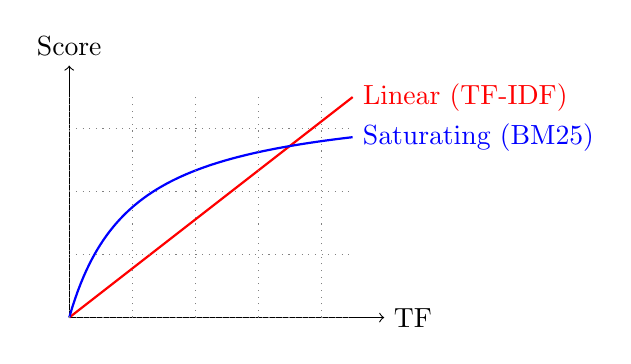
\begin{tikzpicture}[scale=0.8]
    % Axes
    \draw[->] (0,0) -- (5,0) node[right] {TF};
    \draw[->] (0,0) -- (0,4) node[above] {Score};
    
    % Linear (TF-IDF)
    \draw[red, thick] (0,0) -- (4.5,3.5) node[right] {Linear (TF-IDF)};
    
    % Saturating (BM25)
    \draw[blue, thick, domain=0:4.5, samples=100] 
        plot (\x, {3.5*\x/(1+\x)}) node[right] {Saturating (BM25)};
    
    % Grid
    \draw[gray, dotted] (0,0) grid (4.5,3.5);
\end{tikzpicture}
\end{column}
\end{columns}

\vspace{1em}

\begin{alertblock}{Need}
Non-linear TF component that saturates gracefully
\end{alertblock}
\end{frame}

\begin{frame}{BM25 Formula}
\begin{block}{Complete Formula}
$$\text{BM25}(q,d) = \sum_{t \in q} \text{IDF}(t) \cdot \frac{f(t,d) \cdot (k_1+1)}{f(t,d) + k_1 \cdot \left(1-b+b \cdot \frac{|d|}{\text{avgdl}}\right)}$$
\end{block}

\vspace{1em}

\textbf{Three components:}
\begin{enumerate}
    \item \textbf{IDF:} Term importance (like TF-IDF)
    \item \textbf{Saturating TF:} Non-linear term frequency
    \item \textbf{Length normalization:} Penalize long documents
\end{enumerate}

\vspace{1em}

\begin{center}
\textbf{Standard parameters: $k_1 = 1.2$, $b = 0.75$}
\end{center}
\end{frame}

\begin{frame}{BM25 Component 1: IDF}
\begin{block}{IDF Formula}
$$\text{IDF}(t) = \log\frac{N - \text{df}_t + 0.5}{\text{df}_t + 0.5}$$
\end{block}

where:
\begin{itemize}
    \item $N$ = total number of documents
    \item $\text{df}_t$ = document frequency of term $t$
\end{itemize}

\vspace{1em}

\textbf{Properties:}
\begin{itemize}
    \item Similar to TF-IDF but probabilistically motivated
    \item Can be negative for very common terms ($\text{df} > N/2$)
    \item Rare terms get high positive IDF
    \item Common terms get low or negative IDF
\end{itemize}
\end{frame}

\begin{frame}{BM25 Component 2: Saturating TF}
\begin{block}{Saturating TF Formula}
$$\frac{f(t,d) \cdot (k_1+1)}{f(t,d) + k_1}$$
\end{block}

\textbf{Parameter $k_1$ (typically 1.2--2.0):}
\begin{itemize}
    \item $k_1 \to 0$: Boolean matching (TF doesn't matter)
    \item $k_1 \to \infty$: Linear TF (like TF-IDF)
    \item $k_1 = 1.2$: Moderate saturation (standard)
\end{itemize}

\vspace{1em}

\begin{columns}
\begin{column}{0.5\textwidth}
\small
\begin{tabular}{ccc}
\toprule
\textbf{TF} \& \textbf{$k_1=1.2$} \& \textbf{$k_1=2.0$} \\
\midrule
1 \& 0.55 \& 0.67 \\
5 \& 1.53 \& 1.67 \\
10 \& 1.79 \& 1.83 \\
50 \& 1.98 \& 1.96 \\
\bottomrule
\end{tabular}
\end{column}

\begin{column}{0.5\textwidth}
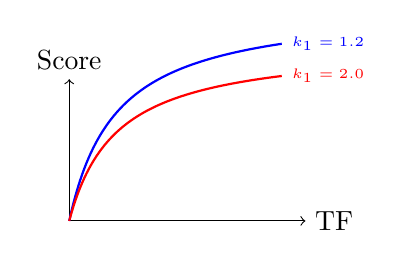
\begin{tikzpicture}[scale=0.6]
    \draw[->] (0,0) -- (5,0) node[right] {TF};
    \draw[->] (0,0) -- (0,3) node[above] {Score};
    
    \draw[blue, thick, domain=0:4.5, samples=100] 
        plot (\x, {2.5*\x*2.2/(1.2*\x+1.2)}) node[right] {\tiny $k_1=1.2$};
    \draw[red, thick, domain=0:4.5, samples=100] 
        plot (\x, {2.5*\x*3/(2*\x+2)}) node[right] {\tiny $k_1=2.0$};
\end{tikzpicture}
\end{column}
\end{columns}
\end{frame}

\begin{frame}{BM25 Component 3: Length Normalization}
\begin{block}{Length Normalization Term}
$$1 - b + b \cdot \frac{|d|}{\text{avgdl}}$$
\end{block}

\textbf{Parameter $b$ (typically 0.75):}
\begin{itemize}
    \item $b = 0$: No length normalization
    \item $b = 1$: Full normalization (penalize long docs heavily)
    \item $b = 0.75$: Partial normalization (standard)
\end{itemize}

\vspace{1em}

\textbf{Why needed:}
\begin{itemize}
    \item Long documents have more terms just by chance
    \item Should we penalize or not? Depends on collection
    \item $b$ controls the trade-off
\end{itemize}
\end{frame}

\begin{frame}{BM25 Example: Effect of Document Length}
\textbf{Scenario:} Term appears 20 times, $k_1=1.2$, $b=0.75$, avgdl=1000

\vspace{1em}

\begin{columns}
\begin{column}{0.5\textwidth}
\textbf{Short Document (500 words)}
\begin{align*}
\text{norm} &= 1 - 0.75 + 0.75 \cdot \frac{500}{1000} \\
&= 0.625 \\
\text{TF component} &= \frac{20 \cdot 2.2}{20 + 1.2 \cdot 0.625} \\
&= \frac{44}{20.75} = 2.12
\end{align*}
\end{column}

\begin{column}{0.5\textwidth}
\textbf{Long Document (2000 words)}
\begin{align*}
\text{norm} &= 1 - 0.75 + 0.75 \cdot \frac{2000}{1000} \\
&= 1.75 \\
\text{TF component} &= \frac{20 \cdot 2.2}{20 + 1.2 \cdot 1.75} \\
&= \frac{44}{22.1} = 1.99
\end{align*}
\end{column}
\end{columns}

\vspace{1em}

\begin{alertblock}{Observation}
Same TF, but short document scores higher due to length penalty
\end{alertblock}
\end{frame}

\begin{frame}{BM25 Example: Rare vs. Common Terms}
\textbf{Collection:} $N = 100{,}000$ documents

\vspace{1em}

\begin{table}
\centering
\begin{tabular}{lccc}
\toprule
\textbf{Term} \& \textbf{df} \& \textbf{IDF} \& \textbf{Interpretation} \\
\midrule
quantum \& 100 \& 6.21 \& Very discriminative \\
algorithm \& 5{,}000 \& 2.99 \& Moderately discriminative \\
system \& 50{,}000 \& -0.41 \& Not discriminative \\
the \& 99{,}000 \& -6.21 \& Actively harmful \\
\bottomrule
\end{tabular}
\end{table}

\vspace{1em}

\begin{block}{Key Insight}
IDF difference drives discrimination:
\begin{itemize}
    \item Rare terms dominate scoring
    \item Common terms contribute little or negatively
    \item Matches on ``quantum'' worth 15$\times$ matches on ``system''
\end{itemize}
\end{block}
\end{frame}

\begin{frame}{BM25 Parameter Tuning Guidelines}
\begin{block}{Standard Defaults}
$k_1 = 1.2$, $b = 0.75$ (works well for many collections)
\end{block}

\vspace{1em}

\begin{columns}
\begin{column}{0.5\textwidth}
\textbf{When to adjust $k_1$:}
\begin{itemize}
    \item \textbf{Verbose collections} (news, articles) \\
    $\rightarrow$ Higher $k_1$ (1.5--2.0)
    \item \textbf{Keyword collections} (tweets, queries) \\
    $\rightarrow$ Lower $k_1$ (0.8--1.2)
\end{itemize}
\end{column}

\begin{column}{0.5\textwidth}
\textbf{When to adjust $b$:}
\begin{itemize}
    \item \textbf{Variable-length docs} (web pages) \\
    $\rightarrow$ Higher $b$ (0.8--0.9)
    \item \textbf{Uniform-length docs} (abstracts) \\
    $\rightarrow$ Lower $b$ (0.5--0.7)
\end{itemize}
\end{column}
\end{columns}

\vspace{1em}

\begin{alertblock}{In Lecture 6 (Learning to Rank)}
You'll learn to tune these parameters systematically using labeled data
\end{alertblock}
\end{frame}

% ====================================================================
% SECTION 3: QUERY EXPANSION
% ====================================================================
\section{Query Expansion and Pseudo Relevance Feedback}

\begin{frame}{The Vocabulary Mismatch Problem}
\begin{exampleblock}{Core Issue}
Queries and relevant documents use different vocabulary:
\end{exampleblock}

\vspace{1em}

\begin{columns}
\begin{column}{0.48\textwidth}
\textbf{Medical Domain}
\begin{itemize}
    \item Query: ``heart attack''
    \item Document: ``myocardial infarction''
\end{itemize}

\vspace{0.5em}

\textbf{Technical Domain}
\begin{itemize}
    \item Query: ``ML''
    \item Document: ``machine learning''
\end{itemize}
\end{column}

\begin{column}{0.48\textwidth}
\textbf{General Domain}
\begin{itemize}
    \item Query: ``elderly care''
    \item Document: ``geriatric nursing''
\end{itemize}

\vspace{0.5em}

\textbf{Result}
\begin{itemize}
    \item BM25 score = 0
    \item Relevant doc not retrieved
\end{itemize}
\end{column}
\end{columns}

\vspace{1em}

\begin{alertblock}{Sparse Retrieval Limitation}
Exact term matching only --- no semantic understanding
\end{alertblock}

\vspace{0.5em}

\textit{(This will be fully solved by Dense Retrieval in Lecture 5)}
\end{frame}

\begin{frame}{Relevance Feedback Overview}
\begin{block}{Explicit Relevance Feedback}
User marks documents as relevant/non-relevant
\begin{itemize}
    \item \textcolor{red}{\ding{55}} Impractical: users won't give feedback
    \item \textcolor{red}{\ding{55}} Chicken-and-egg: need good initial results
\end{itemize}
\end{block}

\vspace{1em}

\begin{block}{Pseudo Relevance Feedback (PRF)}
\textbf{Assumption:} Top-$k$ retrieved documents are relevant
\begin{itemize}
    \item \textcolor{green}{\checkmark} No user interaction needed
    \item \textcolor{green}{\checkmark} Automatic query expansion
    \item \textcolor{red}{\ding{55}} Risk: If assumption fails $\rightarrow$ query drift
\end{itemize}
\end{block}

\vspace{1em}

\textbf{Process:}
\begin{enumerate}
    \item Retrieve initial results with original query
    \item Extract terms from top-$k$ documents
    \item Expand query with these terms
    \item Re-retrieve with expanded query
\end{enumerate}
\end{frame}

\begin{frame}{Rocchio Algorithm}
\begin{block}{Historical Context}
Classic PRF method from 1971, vector space approach
\end{block}

\begin{block}{Formula}
$$\vec{q}_{\text{new}} = \alpha \vec{q}_{\text{original}} + \beta \frac{1}{|R|}\sum_{d \in R} \vec{d} - \gamma \frac{1}{|NR|}\sum_{d \in NR} \vec{d}$$
\end{block}

\textbf{Parameters:}
\begin{itemize}
    \item $\alpha = 1$: Keep original query (always)
    \item $\beta = 0.75$: Weight toward positive examples
    \item $\gamma = 0.15$: Weight away from negative examples
    \item In PRF: $\gamma = 0$ (no negative feedback available)
\end{itemize}

\vspace{1em}

\textbf{Geometric Intuition:}
\begin{itemize}
    \item Move query vector toward centroid of relevant documents
    \item Move away from non-relevant (if available)
\end{itemize}
\end{frame}

\begin{frame}{Rocchio: Geometric Intuition}
\begin{center}
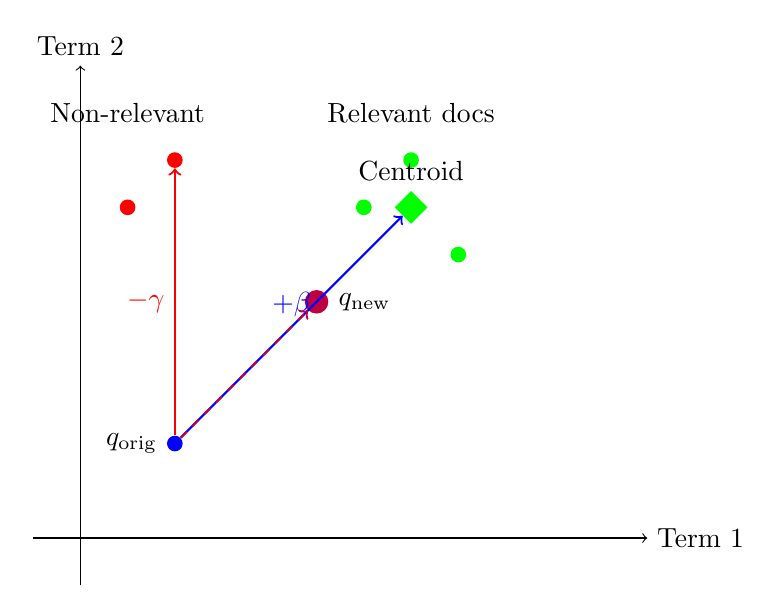
\begin{tikzpicture}[scale=1.2]
    % Axes
    \draw[->] (-0.5,0) -- (6,0) node[right] {Term 1};
    \draw[->] (0,-0.5) -- (0,5) node[above] {Term 2};
    
    % Original query
    \node[circle, fill=blue, inner sep=2pt, label=left:$q_{\text{orig}}$] (q) at (1,1) {};
    
    % Relevant documents
    \node[circle, fill=green, inner sep=2pt] (d1) at (3,3.5) {};
    \node[circle, fill=green, inner sep=2pt] (d2) at (4,3) {};
    \node[circle, fill=green, inner sep=2pt] (d3) at (3.5,4) {};
    \node at (3.5,4.5) {Relevant docs};
    
    % Centroid
    \node[diamond, fill=green, inner sep=3pt, label=above:Centroid] (c) at (3.5,3.5) {};
    
    % Non-relevant documents
    \node[circle, fill=red, inner sep=2pt] (n1) at (1,4) {};
    \node[circle, fill=red, inner sep=2pt] (n2) at (0.5,3.5) {};
    \node at (0.5,4.5) {Non-relevant};
    
    % New query
    \node[circle, fill=purple, inner sep=3pt, label=right:$q_{\text{new}}$] (qn) at (2.5,2.5) {};
    
    % Arrows
    \draw[->, thick, blue] (q) -- (c) node[midway, above] {$+\beta$};
    \draw[->, thick, red] (q) -- (n1) node[midway, left] {$-\gamma$};
    \draw[->, thick, purple, dashed] (q) -- (qn);
\end{tikzpicture}
\end{center}

\textbf{Movement:} Original query shifts toward relevant docs, away from non-relevant
\end{frame}

\begin{frame}{Rocchio Limitations}
\begin{alertblock}{\ding{55} Why Not Standard Anymore?}
\begin{enumerate}
    \item \textbf{Requires vector space representation}
    \begin{itemize}
        \item All terms contribute (even noisy ones)
        \item No principled term selection
    \end{itemize}
    
    \item \textbf{No probabilistic foundation}
    \begin{itemize}
        \item Weights based on geometry, not probability
        \item Harder to interpret
    \end{itemize}
    
    \item \textbf{Empirically outperformed}
    \begin{itemize}
        \item RM3 achieves better results
        \item Probabilistic methods more robust
    \end{itemize}
\end{enumerate}
\end{alertblock}

\vspace{1em}

\begin{block}{Modern Usage}
Mainly historical importance --- good to know the name and concept, but RM3 is the standard
\end{block}
\end{frame}

\begin{frame}{RM3: Relevance Model 3}
\begin{block}{Foundation}
Probabilistic query expansion using language modeling framework
\end{block}

\vspace{1em}

\textbf{Two-stage process:}

\begin{enumerate}
    \item \textbf{Estimate Relevance Model}
    $$P(w|R) \propto \sum_{d \in R} P(w|d) \cdot P(d|q)$$
    \begin{itemize}
        \item For each word $w$, estimate probability from ``relevance''
        \item Weight by how relevant each doc appears: $P(d|q)$ from initial retrieval
        \item Select top \texttt{fb\_terms} words by $P(w|R)$
    \end{itemize}
    
    \item \textbf{Interpolate with Original Query}
    $$P(w|Q_{\text{new}}) = (1-\lambda) \cdot P(w|Q_{\text{original}}) + \lambda \cdot P(w|R)$$
    \begin{itemize}
        \item $\lambda$ typically 0.5--0.8: balance original vs. expansion
    \end{itemize}
\end{enumerate}
\end{frame}

\begin{frame}{RM3: Key Parameters}
\begin{block}{fb\_docs (Feedback Documents): 3--10}
How many top documents to use for expansion
\begin{itemize}
    \item \textbf{Too few:} May miss relevant terms
    \item \textbf{Too many:} Risk including non-relevant documents
    \item \textbf{Standard:} 10
\end{itemize}
\end{block}

\begin{block}{fb\_terms (Feedback Terms): 10--20}
How many expansion terms to add
\begin{itemize}
    \item \textbf{Too few:} Limited expansion benefit
    \item \textbf{Too many:} Noise from marginally relevant terms
    \item \textbf{Standard:} 10
\end{itemize}
\end{block}

\begin{block}{$\lambda$ (Interpolation Weight): 0.5--0.8}
Original vs. expansion weight
\begin{itemize}
    \item \textbf{Lower (0.5):} Trust original query more
    \item \textbf{Higher (0.8):} Trust expansion more
\end{itemize}
\end{block}
\end{frame}

\begin{frame}{RM3 Example}
\textbf{Original Query:} ``machine learning''

\vspace{1em}

\textbf{Top-3 Retrieved Documents (fb\_docs=3):}
\begin{enumerate}
    \item ``Neural networks and deep learning algorithms...''
    \item ``Supervised machine learning techniques...''
    \item ``Machine learning applications in AI...''
\end{enumerate}

\vspace{1em}

\textbf{Extracted Terms (fb\_terms=5):}
\begin{itemize}
    \item neural (P=0.15)
    \item deep (P=0.12)
    \item supervised (P=0.10)
    \item algorithms (P=0.09)
    \item AI (P=0.08)
\end{itemize}

\vspace{1em}

\textbf{Expanded Query ($\lambda=0.6$):}
\\
``machine learning neural deep supervised algorithms AI''
\end{frame}

\begin{frame}{Rocchio vs. RM3}
\begin{table}
\centering
\small
\begin{tabular}{lll}
\toprule
\textbf{Aspect} \& \textbf{Rocchio} \& \textbf{RM3} \\
\midrule
Foundation \& Geometric (vector space) \& Probabilistic (LM) \\
Term selection \& All terms (weighted) \& Top-k by probability \\
Weighting \& Vector magnitude \& $P(w|R)$ \\
Interpretability \& Geometric intuition \& Probabilistic \\
Performance \& Good \& Better \\
Usage today \& Historical \& Standard \\
\bottomrule
\end{tabular}
\end{table}

\vspace{1em}

\begin{block}{Why RM3 Wins}
\begin{itemize}
    \item Probabilistic foundation (principled)
    \item Selective term addition (only strong associations)
    \item Better empirical performance
    \item Standard in modern systems (Indri, Anserini, Pyterrier)
\end{itemize}
\end{block}
\end{frame}

\begin{frame}{When Query Expansion Helps vs. Hurts}
\begin{columns}
\begin{column}{0.48\textwidth}
\begin{block}{\checkmark Helps When:}
\begin{itemize}
    \item Initial results mostly relevant
    \item Vocabulary mismatch present
    \item Broad informational queries
    \item Query: ``climate change''
    \item Expansion adds: ``warming'', ``CO2'', ``emissions''
\end{itemize}
\end{block}
\end{column}

\begin{column}{0.48\textwidth}
\begin{alertblock}{\ding{55} Hurts When:}
\begin{itemize}
    \item Initial results off-topic
    \item Ambiguous queries
    \item Very specific queries
    \item Query: ``jaguar''
    \item Expansion adds: ``car'', ``speed'' (wrong sense!)
\end{itemize}
\end{alertblock}
\end{column}
\end{columns}

\vspace{1em}

\begin{exampleblock}{Query Drift Example}
\textbf{Query:} ``python programming''

\textbf{Top result:} Article about Python snake species

\textbf{Expansion:} ``reptile'', ``snake'', ``habitat'', ``venom''

\textbf{Result:} Completely wrong direction!
\end{exampleblock}
\end{frame}

% ====================================================================
% SECTION 4: LANGUAGE MODELS
% ====================================================================
\section{Statistical Language Models for Ranking}

\begin{frame}{A Different Ranking Philosophy}
\begin{columns}
\begin{column}{0.48\textwidth}
\textbf{BM25 Approach:}
\begin{itemize}
    \item ``How well does document match query?''
    \item Scoring based on term overlap
    \item Weighted by importance (IDF, TF)
\end{itemize}

\vspace{1em}

\begin{block}{Matching Score}
$$\text{score}(q,d) = \sum_{t} w(t,q,d)$$
\end{block}
\end{column}

\begin{column}{0.48\textwidth}
\textbf{Language Model Approach:}
\begin{itemize}
    \item ``How likely would this document generate this query?''
    \item Rank by $P(q|d)$
    \item Probabilistic generative model
\end{itemize}

\vspace{1em}

\begin{block}{Generative Probability}
$$\text{score}(q,d) = P(q|d)$$
\end{block}
\end{column}
\end{columns}

\vspace{1em}

\begin{exampleblock}{Generative Story}
\begin{enumerate}
    \item Pick a document $d$
    \item Document has a language model (probability distribution over words)
    \item Generate query by sampling from this distribution
    \item Documents that would more likely generate $q$ are ranked higher
\end{enumerate}
\end{exampleblock}
\end{frame}

\begin{frame}{Why Language Models Matter}
\begin{block}{Principled Probabilistic Framework}
\begin{itemize}
    \item Solid theoretical foundation (compared to heuristic weighting)
    \item Smoothing becomes natural and essential
    \item Interpretable as generative process
\end{itemize}
\end{block}

\vspace{1em}

\begin{block}{Connection to Modern IR}
\begin{itemize}
    \item Foundation for neural language models (Lecture 4)
    \item BERT, GPT are sophisticated language models
    \item Understanding statistical LMs helps understand neural LMs
\end{itemize}
\end{block}

\vspace{1em}

\begin{alertblock}{Preview}
In Lecture 4, we'll see how transformers extend this probabilistic foundation with contextualized representations
\end{alertblock}
\end{frame}

\begin{frame}{Query Likelihood Model}
\begin{block}{Basic Formulation}
Rank documents by probability they would generate the query:
$$P(q|d) = \prod_{w \in q} P(w|d)^{\text{count}(w,q)}$$
\end{block}

\vspace{1em}

\textbf{Maximum Likelihood Estimate:}
$$P_{\text{ML}}(w|d) = \frac{\text{count}(w,d)}{|d|}$$

\vspace{1em}

\begin{alertblock}{Critical Problem: Zero Probabilities}
If query word doesn't appear in document:
\begin{itemize}
    \item $P(w|d) = 0$
    \item Product $\rightarrow$ entire $P(q|d) = 0$
    \item Document ranked at bottom even if partially relevant
\end{itemize}
\end{alertblock}

\textbf{Solution:} Smoothing is essential, not optional!
\end{frame}

\begin{frame}{Zero Probability Example}
\textbf{Query:} ``machine learning algorithms''

\vspace{0.5em}

\textbf{Document:} ``This paper presents a novel neural network approach to supervised machine learning.''

\vspace{1em}

\begin{table}
\centering
\begin{tabular}{lccc}
\toprule
\textbf{Term} \& \textbf{count(w,d)} \& \textbf{$P_{\text{ML}}(w|d)$} \& \textbf{Result} \\
\midrule
machine \& 1 \& $1/15 = 0.067$ \& \checkmark \\
learning \& 1 \& $1/15 = 0.067$ \& \checkmark \\
algorithms \& 0 \& $0/15 = 0$ \& \textcolor{red}{\ding{55} ZERO!} \\
\midrule
$P(q|d)$ \& \multicolumn{3}{c}{$0.067 \times 0.067 \times 0 = \mathbf{0}$} \\
\bottomrule
\end{tabular}
\end{table}

\vspace{1em}

\begin{alertblock}{Problem}
Document is clearly relevant, but one missing term kills the entire score!
\end{alertblock}
\end{frame}

\begin{frame}{Smoothing: Core Idea}
\begin{block}{Principle}
Mix document evidence with collection evidence:
$$P(w|d) = f(\text{document evidence}, \text{collection evidence})$$
\end{block}

\vspace{1em}

\textbf{Collection Language Model:}
$$P(w|C) = \frac{\sum_{d' \in C} \text{count}(w,d')}{\sum_{d' \in C} |d'|}$$

\vspace{1em}

\textbf{Two Main Approaches:}
\begin{enumerate}
    \item \textbf{Jelinek-Mercer:} Fixed linear interpolation
    \item \textbf{Dirichlet:} Length-adaptive interpolation
\end{enumerate}

\vspace{1em}

\begin{exampleblock}{Effect}
Even if $\text{count}(w,d) = 0$, we have $P(w|d) > 0$ from collection
\end{exampleblock}
\end{frame}

\begin{frame}{Jelinek-Mercer Smoothing}
\begin{block}{Formula}
$$P(w|d) = (1-\lambda) \cdot P_{\text{ML}}(w|d) + \lambda \cdot P(w|C)$$
\end{block}

\textbf{Parameter $\lambda$ (typically 0.1--0.3):}
\begin{itemize}
    \item How much to trust collection vs. document
    \item $\lambda = 0$: Only use document (no smoothing)
    \item $\lambda = 1$: Only use collection (ignore document)
    \item $\lambda = 0.1$: Mostly trust document, small collection backup
\end{itemize}

\vspace{1em}

\textbf{Properties:}
\begin{itemize}
    \item \textcolor{green}{\checkmark} Simple and interpretable
    \item \textcolor{green}{\checkmark} Same $\lambda$ for all documents
    \item \textcolor{red}{\ding{55}} Doesn't adapt to document length
\end{itemize}
\end{frame}

\begin{frame}{Dirichlet Smoothing}
\begin{block}{Formula}
$$P(w|d) = \frac{\text{count}(w,d) + \mu \cdot P(w|C)}{|d| + \mu}$$
\end{block}

\textbf{Parameter $\mu$ (typically 1000--2500):}
\begin{itemize}
    \item Smoothing strength (number of ``pseudo-counts'' from collection)
    \item Higher $\mu$: More smoothing (trust collection more)
    \item Lower $\mu$: Less smoothing (trust document more)
\end{itemize}

\vspace{1em}

\textbf{Key Difference: Length-Adaptive}
\begin{itemize}
    \item \textbf{Short documents:} $\mu$ dominates denominator $\rightarrow$ rely more on collection
    \item \textbf{Long documents:} Actual counts dominate $\rightarrow$ rely on document
    \item Automatically adapts smoothing to document length!
\end{itemize}
\end{frame}

\begin{frame}{Dirichlet Smoothing: Length Adaptation Example}
\textbf{Term ``algorithm'' with $P(w|C) = 0.001$, $\mu = 2000$}

\vspace{1em}

\begin{table}
\centering
\begin{tabular}{lccc}
\toprule
\textbf{Document} \& \textbf{count(w,d)} \& \textbf{$|d|$} \& \textbf{$P(w|d)$} \\
\midrule
Short doc \& 2 \& 100 \& $\frac{2 + 2000 \times 0.001}{100 + 2000} = \frac{4}{2100} = 0.0019$ \\
\midrule
Long doc \& 2 \& 2000 \& $\frac{2 + 2000 \times 0.001}{2000 + 2000} = \frac{4}{4000} = 0.001$ \\
\bottomrule
\end{tabular}
\end{table}

\vspace{1em}

\begin{block}{Observation}
\begin{itemize}
    \item Same term count (2 occurrences)
    \item Short doc gets higher probability (less smoothing needed)
    \item Long doc gets more smoothing (closer to collection probability)
    \item This is \textbf{automatic} based on $|d|$
\end{itemize}
\end{block}
\end{frame}

\begin{frame}{Jelinek-Mercer vs. Dirichlet}
\begin{table}
\centering
\small
\begin{tabular}{lll}
\toprule
\textbf{Aspect} \& \textbf{Jelinek-Mercer} \& \textbf{Dirichlet} \\
\midrule
Formula \& $(1-\lambda) P_{\text{ML}}(w|d) + \lambda P(w|C)$ \& $\frac{\text{count}(w,d) + \mu P(w|C)}{|d| + \mu}$ \\
Parameter \& $\lambda$ (0.1--0.3) \& $\mu$ (1000--2500) \\
Length adaptation \& Fixed for all docs \& Automatic \\
Smoothing amount \& Same for all docs \& More for short docs \\
Interpretation \& Linear interpolation \& Pseudo-counts \\
Best for \& Uniform-length collections \& Variable-length collections \\
\bottomrule
\end{tabular}
\end{table}

\vspace{1em}

\begin{block}{Which to Use?}
\begin{itemize}
    \item \textbf{Dirichlet generally better} for most collections
    \item Standard in Indri, Galago search engines
    \item But requires tuning $\mu$
\end{itemize}
\end{block}
\end{frame}

\begin{frame}{Language Models vs. BM25}
\begin{table}
\centering
\small
\begin{tabular}{lll}
\toprule
\textbf{Aspect} \& \textbf{BM25} \& \textbf{Language Models} \\
\midrule
Philosophy \& Term matching score \& Generative probability \\
TF handling \& Explicit saturation $(k_1)$ \& Implicit via smoothing \\
Length norm \& Explicit $(b)$ \& Implicit via smoothing \\
IDF \& Explicit component \& Through $P(w|C)$ \\
Zero probabilities \& Avoided via IDF \& Smoothing essential \\
Parameters \& $k_1, b$ \& $\lambda$ or $\mu$ \\
Foundation \& Probabilistic relevance \& Language modeling \\
\bottomrule
\end{tabular}
\end{table}

\vspace{1em}

\begin{block}{Practical Comparison}
\begin{itemize}
    \item With appropriate parameters, rankings often similar
    \item BM25: Better understood, more robust defaults
    \item Dirichlet LM: Better for variable-length collections
    \item \textbf{Best practice:} Try both!
\end{itemize}
\end{block}
\end{frame}

\begin{frame}{Connection: RM3 Uses Language Modeling}
\begin{block}{Recall RM3 Formula}
$$P(w|R) \propto \sum_{d \in R} P(w|d) \cdot P(d|q)$$
\end{block}

\vspace{1em}

\textbf{Key Insight:}
\begin{itemize}
    \item RM3 uses language modeling framework
    \item $P(w|d)$ estimated for each pseudo-relevant doc
    \item Expansion terms selected by $P(w|R)$
    \item RM3 builds a \textit{language model of relevance}
\end{itemize}

\vspace{1em}

\begin{exampleblock}{Why This Matters}
Understanding language models helps you understand query expansion:
\begin{itemize}
    \item Both use probabilistic term distributions
    \item Both require smoothing
    \item Natural progression: LM $\rightarrow$ RM3 $\rightarrow$ Neural LM (Lecture 4)
\end{itemize}
\end{exampleblock}
\end{frame}

% ====================================================================
% SECTION 5: PYTERRIER
% ====================================================================
\section{Hands-On with PyTerrier}

\begin{frame}[fragile]{PyTerrier Setup}
\begin{lstlisting}[language=Python]
import pyterrier as pt
if not pt.started():
    pt.init()

# Load dataset (VASWANI: small, fast for teaching)
dataset = pt.get_dataset('irds:vaswani')

# Index (or use pre-built)
if not os.path.exists("./vaswani_index"):
    indexer = pt.IterDictIndexer("./vaswani_index")
    index_ref = indexer.index(dataset.get_corpus_iter())
else:
    index_ref = pt.IndexRef.of("./vaswani_index")

index = pt.IndexFactory.of(index_ref)

# Get topics and qrels
topics = dataset.get_topics().head(10)  # Subset for speed
qrels = dataset.get_qrels()
\end{lstlisting}
\end{frame}

\begin{frame}[fragile]{Exercise 1: BM25 Baseline}
\begin{lstlisting}[language=Python]
# Default BM25 (k1=1.2, b=0.75)
bm25 = pt.BatchRetrieve(index, wmodel="BM25")

# Retrieve results
results = bm25.transform(topics)

# Examine one query
print(results[results['qid']=='1'][['qid', 'docno', 'score', 'rank']].head())
\end{lstlisting}

\vspace{1em}

\textbf{Output:}
\begin{table}
\tiny
\begin{tabular}{llcc}
\toprule
qid \& docno \& score \& rank \\
\midrule
1 \& 51 \& 8.234 \& 1 \\
1 \& 486 \& 7.921 \& 2 \\
1 \& 12 \& 7.456 \& 3 \\
\bottomrule
\end{tabular}
\end{table}
\end{frame}

\begin{frame}[fragile]{Exercise 1: Parameter Effects}
\begin{lstlisting}[language=Python]
# Create BM25 variants
bm25_default = pt.BatchRetrieve(index, wmodel="BM25")
bm25_high_k1 = pt.BatchRetrieve(index, wmodel="BM25", 
                                 controls={"bm25.k1": "2.0"})
bm25_low_b = pt.BatchRetrieve(index, wmodel="BM25", 
                               controls={"bm25.b": "0.3"})
bm25_high_b = pt.BatchRetrieve(index, wmodel="BM25", 
                                controls={"bm25.b": "0.95"})

# Compare
comparison = pt.Experiment(
    [bm25_default, bm25_high_k1, bm25_low_b, bm25_high_b],
    topics, qrels,
    eval_metrics=["map", "ndcg_cut_10", "P_10"],
    names=["Default", "k1=2.0", "b=0.3", "b=0.95"]
)
print(comparison)
\end{lstlisting}
\end{frame}

\begin{frame}[fragile]{Exercise 2: RM3 Query Expansion}
\begin{lstlisting}[language=Python]
# RM3 pipeline: retrieve -> expand -> retrieve again
bm25 = pt.BatchRetrieve(index, wmodel="BM25")
rm3 = pt.rewrite.RM3(index)  # Default: fb_docs=10, fb_terms=10
pipeline_rm3 = bm25 >> rm3 >> bm25

# Compare with baseline
comparison = pt.Experiment(
    [bm25, pipeline_rm3],
    topics, qrels,
    eval_metrics=["map", "ndcg_cut_10", "recall_100"],
    names=["BM25", "BM25+RM3"]
)
print(comparison)

# Inspect expanded query
expanded = rm3.transform(topics)
print("Original:", topics[topics['qid']=='1']['query'].values[0])
print("Expanded:", expanded[expanded['qid']=='1']['query'].values[0])
\end{lstlisting}
\end{frame}

\begin{frame}[fragile]{Exercise 2: RM3 Parameter Tuning}
\begin{lstlisting}[language=Python]
# Try different RM3 configurations
rm3_configs = {
    "RM3 (default)": pt.rewrite.RM3(index),
    "RM3 (5 docs)": pt.rewrite.RM3(index, fb_docs=5),
    "RM3 (15 docs)": pt.rewrite.RM3(index, fb_docs=15),
    "RM3 (5 terms)": pt.rewrite.RM3(index, fb_terms=5),
    "RM3 (30 terms)": pt.rewrite.RM3(index, fb_terms=30),
}

pipelines = {name: bm25 >> rm3_cfg >> bm25 
             for name, rm3_cfg in rm3_configs.items()}

results = pt.Experiment(
    [bm25] + list(pipelines.values()),
    topics, qrels,
    eval_metrics=["map", "ndcg_cut_10"],
    names=["BM25"] + list(pipelines.keys())
)
\end{lstlisting}
\end{frame}

\begin{frame}[fragile]{Exercise 3: Language Models}
\begin{lstlisting}[language=Python]
# Dirichlet LM with different mu values
lm_1000 = pt.BatchRetrieve(index, wmodel="DirichletLM", 
                           controls={"c": "1000"})
lm_2500 = pt.BatchRetrieve(index, wmodel="DirichletLM", 
                           controls={"c": "2500"})  # default
lm_5000 = pt.BatchRetrieve(index, wmodel="DirichletLM", 
                           controls={"c": "5000"})

# Compare with BM25
comparison = pt.Experiment(
    [bm25, lm_1000, lm_2500, lm_5000],
    topics, qrels,
    eval_metrics=["map", "ndcg_cut_10", "P_10"],
    names=["BM25", "LM (mu=1000)", "LM (mu=2500)", "LM (mu=5000)"]
)
print(comparison)
\end{lstlisting}
\end{frame}

\begin{frame}[fragile]{Exercise 4: Comprehensive Comparison}
\begin{lstlisting}[language=Python]
# Build all systems
systems = {
    "BM25": bm25,
    "Dirichlet LM": lm_2500,
    "BM25 + RM3": bm25 >> pt.rewrite.RM3(index) >> bm25,
    "LM + RM3": lm_2500 >> pt.rewrite.RM3(index) >> lm_2500,
}

# Final evaluation
final_results = pt.Experiment(
    list(systems.values()),
    topics, qrels,
    eval_metrics=["map", "ndcg_cut_10", "P_10", "recall_100"],
    names=list(systems.keys())
)

print(final_results)
\end{lstlisting}

\textbf{Discussion:} Which baseline wins? Does RM3 help more for BM25 or LM?
\end{frame}

\begin{frame}{Hands-On: Student Exercises}
\begin{block}{Exercise 1: BM25 Parameters (5 mins)}
\begin{itemize}
    \item Pick one query
    \item Compare scores for top document across different $b$ values
    \item Find a long document and short document
    \item How does $b$ affect their relative scores?
\end{itemize}
\end{block}

\begin{block}{Exercise 2: Query Expansion Analysis (7 mins)}
\begin{itemize}
    \item Find a query where RM3 helps significantly
    \item Find a query where RM3 hurts (query drift)
    \item Look at expanded terms --- are they semantically related?
    \item What happens with fb\_docs=3 vs. fb\_docs=20?
\end{itemize}
\end{block}

\begin{block}{Exercise 3: BM25 vs. LM (5 mins)}
\begin{itemize}
    \item Find documents where BM25 and LM disagree
    \item Are they long or short documents?
    \item Check document lengths and relate to smoothing
\end{itemize}
\end{block}
\end{frame}

% ====================================================================
% SECTION 6: CONNECTIONS
% ====================================================================
\section{Connections to Future Lectures}

\begin{frame}{What We've Covered Today}
\begin{block}{Sparse, Term-Based Ranking}
\begin{itemize}
    \item \textbf{BM25:} Probabilistic relevance, saturating TF, length normalization
    \item \textbf{Language Models:} Generative probabilities, smoothing essential
    \item \textbf{Query Expansion:} RM3 for vocabulary mismatch
\end{itemize}
\end{block}

\vspace{1em}

\begin{alertblock}{Fundamental Limitations}
\begin{itemize}
    \item Still bag-of-words (order doesn't matter)
    \item Exact term matching only
    \item No semantic understanding
    \item ``car'' and ``automobile'' completely different
    \item ``bank'' (river) vs. ``bank'' (financial) treated identically
\end{itemize}
\end{alertblock}
\end{frame}

\begin{frame}{Preview: Lecture 4 --- Transformer Re-rankers}
\begin{block}{Why Transformers?}
Sparse methods don't understand semantics
\begin{itemize}
    \item Synonyms not recognized
    \item Polysemy not resolved
    \item Context not considered
\end{itemize}
\end{block}

\begin{block}{Solution: Contextualized Embeddings}
\begin{itemize}
    \item BERT: Bidirectional transformer language model
    \item Each word embedding depends on context
    \item ``bank'' near river $\rightarrow$ different embedding than ``bank'' near money
\end{itemize}
\end{block}

\begin{block}{Re-ranking Architecture}
\begin{enumerate}
    \item BM25/LM retrieves 1000 candidates (fast, today's lecture)
    \item BERT re-ranks top 100 (slow but accurate, next lecture)
\end{enumerate}
\end{block}

\textbf{Connection:} Your BM25 pipelines become first-stage retrievers
\end{frame}

\begin{frame}{Preview: Lecture 5 --- Dense Retrieval}
\begin{block}{Why Dense Retrieval?}
Query expansion helps but doesn't eliminate vocabulary mismatch
\begin{itemize}
    \item RM3 adds related terms, but still exact matching
    \item ``elderly care'' and ``geriatric nursing'' still won't match
\end{itemize}
\end{block}

\begin{block}{Solution: Semantic Embeddings}
\begin{itemize}
    \item Embed queries and documents in dense vector space
    \item Similarity measured by dot product or cosine
    \item Semantically similar items close in embedding space
    \item ``elderly care'' $\approx$ ``geriatric nursing'' in embedding space
\end{itemize}
\end{block}

\begin{alertblock}{\ding{55} Trade-off}
\begin{itemize}
    \item \textcolor{green}{\checkmark} No vocabulary gap
    \item \textcolor{red}{\ding{55}} More expensive (requires neural encoding)
    \item \textcolor{red}{\ding{55}} Needs approximate nearest neighbor search
\end{itemize}
\end{alertblock}

\textbf{Connection:} RM3 tries to bridge vocab gap; dense retrieval eliminates it
\end{frame}

\begin{frame}{Preview: Lecture 6 --- Learning to Rank}
\begin{block}{Why Learning to Rank?}
We've been hand-tuning parameters:
\begin{itemize}
    \item BM25: $k_1$, $b$
    \item Language models: $\mu$ or $\lambda$
    \item RM3: fb\_docs, fb\_terms
\end{itemize}
What if we could learn optimal settings from data?
\end{block}

\begin{block}{Solution: Supervised Learning}
\begin{enumerate}
    \item Extract features (BM25 score, LM score, doc length, etc.)
    \item Train model to optimize ranking directly
    \item Common approaches: LambdaMART, RankSVM, LambdaRank
\end{enumerate}
\end{block}

\begin{exampleblock}{Feature Engineering}
All today's methods become features:
\begin{itemize}
    \item BM25(q,d), DirichletLM(q,d), |d|, IDF(q), overlap(q,d), ...
    \item Learn optimal combination from labeled data
\end{itemize}
\end{exampleblock}

\textbf{Connection:} Today's methods are features in LTR
\end{frame}

\begin{frame}{The Modern Retrieval Stack}
\begin{center}
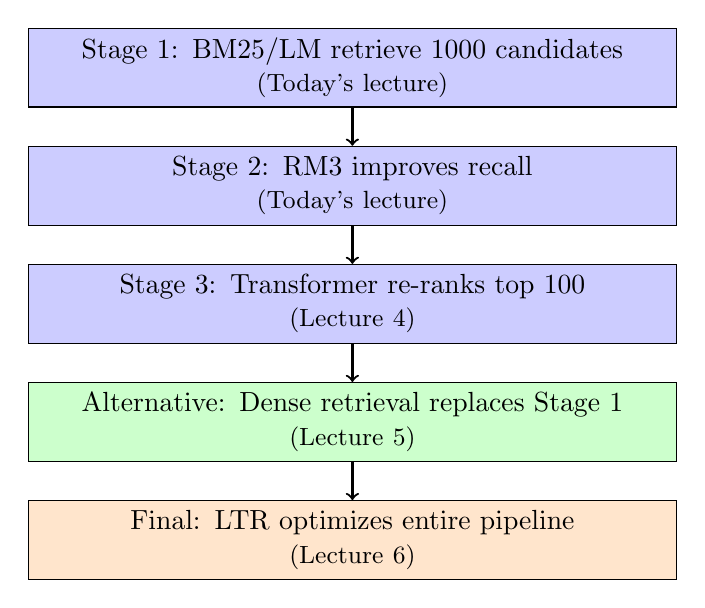
\begin{tikzpicture}[
    node distance=1.5cm,
    box/.style={rectangle, draw, fill=blue!20, text width=8cm, align=center, minimum height=1cm},
    arrow/.style={->, thick}
]
    \node[box] (stage1) {Stage 1: BM25/LM retrieve 1000 candidates \\ \small (Today's lecture)};
    \node[box, below of=stage1] (stage2) {Stage 2: RM3 improves recall \\ \small (Today's lecture)};
    \node[box, below of=stage2] (stage3) {Stage 3: Transformer re-ranks top 100 \\ \small (Lecture 4)};
    \node[box, below of=stage3, fill=green!20] (alt) {Alternative: Dense retrieval replaces Stage 1 \\ \small (Lecture 5)};
    \node[box, below of=alt, fill=orange!20] (final) {Final: LTR optimizes entire pipeline \\ \small (Lecture 6)};
    
    \draw[arrow] (stage1) -- (stage2);
    \draw[arrow] (stage2) -- (stage3);
    \draw[arrow] (stage3) -- (alt);
    \draw[arrow] (alt) -- (final);
\end{tikzpicture}
\end{center}
\end{frame}

\begin{frame}{Why Sparse Methods Still Matter}
\begin{enumerate}
    \item \textbf{Efficiency}
    \begin{itemize}
        \item Orders of magnitude faster than dense retrieval
        \item BM25: microseconds, Dense: milliseconds
        \item Essential for large-scale systems
    \end{itemize}
    
    \item \textbf{Transparency}
    \begin{itemize}
        \item Explainable scores (IDF, TF contributions)
        \item Debuggable (inspect why doc ranked high)
        \item Neural models are black boxes
    \end{itemize}
    
    \item \textbf{Hybrid Systems}
    \begin{itemize}
        \item Best results combine sparse + dense
        \item Sparse catches exact matches, dense catches semantic
        \item Complementary strengths
    \end{itemize}
    
    \item \textbf{First-Stage Retrieval}
    \begin{itemize}
        \item Neural methods too slow for full corpus
        \item BM25 narrows down candidates
        \item Neural re-ranking on top
    \end{itemize}
    
    \item \textbf{Feature Engineering for LTR}
    \begin{itemize}
        \item BM25, LM scores are powerful features
        \item Learning to rank needs good features
    \end{itemize}
\end{enumerate}
\end{frame}

% ====================================================================
% WRAP-UP
% ====================================================================
\section{Summary and Assignment}

\begin{frame}{Key Takeaways}
\begin{block}{1. BM25 is the Industry Standard}
\begin{itemize}
    \item Probabilistic foundation, robust performance
    \item Tune $k_1$ for TF saturation, $b$ for length normalization
    \item Defaults ($k_1=1.2$, $b=0.75$) work well for most collections
\end{itemize}
\end{block}

\begin{block}{2. RM3 Improves Recall}
\begin{itemize}
    \item Addresses vocabulary mismatch via query expansion
    \item Watch for query drift (test on validation set)
    \item Typically improves MAP by 5-15\%
\end{itemize}
\end{block}

\begin{block}{3. Language Models Provide Principled Alternative}
\begin{itemize}
    \item Generative probabilistic framework
    \item Smoothing is essential (handles zero probabilities)
    \item Dirichlet often best for variable-length collections
\end{itemize}
\end{block}

\begin{block}{4. PyTerrier Makes Experimentation Easy}
\begin{itemize}
    \item Pipeline composition: \texttt{bm25 >> rm3 >> bm25}
    \item Built-in evaluation with standard metrics
    \item Use it for your projects!
\end{itemize}
\end{block}
\end{frame}

\begin{frame}{Assignment: Sparse Ranking Comparison}
\textbf{Due:} Before Lecture 5

\vspace{1em}

\begin{block}{Part 1: Baseline Comparison}
\begin{itemize}
    \item Implement BM25 and Dirichlet LM on new collection
    \item Tune parameters: 3+ values each for $k_1$, $b$, $\mu$
    \item Report MAP, NDCG@10, P@10
\end{itemize}
\end{block}

\begin{block}{Part 2: Query Expansion}
\begin{itemize}
    \item Add RM3 to your best baseline
    \item Experiment with fb\_docs (3, 5, 10, 15) and fb\_terms (5, 10, 20)
    \item Identify queries helped vs. hurt by expansion
\end{itemize}
\end{block}

\begin{block}{Part 3: Analysis}
\begin{itemize}
    \item For 3 queries, explain ranking differences between BM25 and LM
    \item Show example of successful query expansion
    \item Show example of query drift
    \item Discuss: When would you use each method in production?
\end{itemize}
\end{block}
\end{frame}

\begin{frame}{Assignment: Looking Ahead}
\begin{block}{Part 4: Connecting to Future Lectures}
Based on your experimental results:
\begin{itemize}
    \item Which queries would benefit most from semantic matching (dense retrieval)?
    \item Which might still need sparse retrieval?
    \item What features would you extract for learning to rank?
\end{itemize}
\end{block}

\vspace{1em}

\begin{alertblock}{Deliverable}
Jupyter notebook with:
\begin{itemize}
    \item Code for all experiments
    \item Results table with all metrics
    \item Written analysis (2-3 pages)
    \item Bring your best BM25/LM pipeline to Lecture 4
\end{itemize}
\end{alertblock}
\end{frame}

\begin{frame}{Next Class: Transformer Re-rankers}
\begin{block}{Preparation}
\textbf{Read:}
\begin{itemize}
    \item Vaswani et al. (2017): ``Attention Is All You Need''
    \item Devlin et al. (2019): ``BERT: Pre-training of Deep Bidirectional Transformers''
\end{itemize}

\vspace{0.5em}

\textbf{Skim:}
\begin{itemize}
    \item Nogueira \& Cho (2019): ``Passage Re-ranking with BERT''
\end{itemize}
\end{block}

\vspace{1em}

\begin{exampleblock}{What We'll Build}
\begin{itemize}
    \item Use your BM25 pipeline as first-stage retriever
    \item Add BERT re-ranker on top
    \item Compare sparse vs. neural ranking
    \item Understand attention mechanisms
\end{itemize}
\end{exampleblock}
\end{frame}

\begin{frame}{Questions?}
\begin{center}
\Huge Questions?

\vspace{2em}

\Large
Office Hours: [Your time]

\vspace{1em}

Email: [Your email]

\vspace{2em}

\normalsize
\textbf{Good luck with the assignment!}
\end{center}
\end{frame}

% Backup slides
\appendix

\begin{frame}{Backup: BM25 Variants}
\begin{block}{BM25+}
Adds query term frequency normalization:
$$\text{BM25+}(q,d) = \sum_{t \in q} \text{IDF}(t) \cdot \left(\frac{f(t,d) \cdot (k_1+1)}{f(t,d) + k_1 \cdot \text{norm}} + \delta\right)$$
\begin{itemize}
    \item $\delta$: Lower bound on term contribution
    \item Not widely adopted in practice
\end{itemize}
\end{block}

\begin{block}{BM25F (Fielded Documents)}
Extends BM25 for documents with multiple fields (title, body, etc.):
\begin{itemize}
    \item Different $k_1$, $b$ per field
    \item Field weights
    \item Common in web search (title more important than body)
\end{itemize}
\end{block}
\end{frame}

\begin{frame}{Backup: Other Smoothing Methods}
\begin{block}{Absolute Discounting}
$$P(w|d) = \frac{\max(\text{count}(w,d) - \delta, 0)}{|d|} + \frac{\delta \cdot |V_d|}{|d|} \cdot P(w|C)$$
\begin{itemize}
    \item Subtracts fixed discount $\delta$ from each count
    \item Redistributes to unseen words
    \item Less common than JM or Dirichlet
\end{itemize}
\end{block}

\begin{block}{Two-Stage Smoothing}
Combine multiple smoothing methods:
\begin{itemize}
    \item Stage 1: Document-level smoothing (Dirichlet)
    \item Stage 2: Collection-level smoothing (JM)
    \item Can improve performance but more complex
\end{itemize}
\end{block}
\end{frame}

\begin{frame}[fragile]{Backup: PyTerrier Advanced Features}
\begin{block}{Custom Weighting Models}
\begin{lstlisting}[language=Python]
# Implement your own weighting model
class MyWeightingModel(pt.Transformer):
    def transform(self, topics):
        # Custom scoring logic
        return results
\end{lstlisting}
\end{block}

\begin{block}{Feature Extraction for LTR}
\begin{lstlisting}[language=Python]
# Extract multiple features
features = pt.FeaturesBatchRetrieve(
    index,
    wmodel="BM25",
    features=["WMODEL:BM25", "WMODEL:DirichletLM", "WMODEL:TF_IDF"]
)
\end{lstlisting}
\end{block}
\end{frame}

\end{document}